\documentclass[12pt, a4paper]{article}

% ------------------------------ font
\usepackage{times} %pdflatex
% \usepackage{luatexja}
% \usepackage{luatexja-fontspec}

% \setmainfont{Times New Roman}
% \setmainjfont[BoldFont=IPAexGothic]{IPAexMincho}
\usepackage{color}
\newcommand{\revise}[1]{{\color{red}{#1}}}

% ------------------------------ math
\usepackage{amsmath,amssymb}
\usepackage{siunitx}

% ------------------------------ author & natbib
\usepackage{authblk}
\usepackage[semicolon]{natbib}
\bibliographystyle{agsm}

% ------------------------------ appendix
\usepackage[title]{appendix}

% ------------------------------ tables
\usepackage{here}
\usepackage{longtable, booktabs, array}
\usepackage{threeparttable, threeparttablex, multirow}
% \newcolumntype{d}{S[input-symbols = ()]}
\usepackage{lscape}

% ------------------------------- figures
\usepackage[labelfont=bf, labelsep=period, justification=justified]{caption}
\usepackage{graphics, graphicx}
\makeatletter
\def\maxwidth{\ifdim\Gin@nat@width>\linewidth\linewidth\else\Gin@nat@width\fi}
\def\maxheight{\ifdim\Gin@nat@height>\textheight\textheight\else\Gin@nat@height\fi}
\makeatother
% Scale images if necessary, so that they will not overflow the page
% margins by default, and it is still possible to overwrite the defaults
% using explicit options in \includegraphics[width, height, ...]{}
\setkeys{Gin}{width=\maxwidth,height=\maxheight,keepaspectratio}

% ------------------------------ page settings
\usepackage[left=3cm,right=3cm,top=3cm,bottom=3cm]{geometry}
\usepackage{setspace}
\renewcommand{\baselinestretch}{2}
\providecommand{\tightlist}{%
  \setlength{\itemsep}{0pt}\setlength{\parskip}{0pt}}

% ------------------------------ hyperlink
\usepackage[hidelinks]{hyperref}

% ------------------------------ other packages
\usepackage{booktabs}
\usepackage{siunitx}

  \newcolumntype{d}{S[
    input-open-uncertainty=,
    input-close-uncertainty=,
    parse-numbers = false,
    table-align-text-pre=false,
    table-align-text-post=false
  ]}
  

% ------------------------------ paper information
\title{Exploring Text Messages to Promote Stem Cell Donation:
Evidence from Field Experiment of Japan Marrow Donor Program\thanks{We would like to thank the Japan Marrow Donor Program Office for managing the field experiment and providing us with the data. This study was conducted with the approval of the institutional review board of the Graduate School of Economics, Osaka University (approval number: R030305-2) and the Japan Marrow Donor Program (approval number: JMDP2021-04). Declarations of interest: none. Funding: This work was supported by the Japan Society for the Promotion of Science {[}grant number 20H05632{]} and the Ministry of Health, Labour and Welfare {[}grant number 19FF1001{]}.}}
\author{}
\date{}

\makeatletter
\renewcommand*{\@fnsymbol}[1]{\ifcase#1\or*\else\@arabic{\numexpr#1-1\relax}\fi}
\makeatother

\begin{document}
\begin{spacing}{1}
  \maketitle
    \clearpage
  \begin{abstract}
  Approximately half of the patients registered with the Japan Marrow Donor Program (JMDP) receive allogeneic hematopoietic stem cell transplantation from JMDP donors. This is because much of transplant coordination is interrupted before the confirmatory typing stage owing to donor-related reasons. A field experiment was conducted in collaboration with JMDP to verify the effects of providing information to increase the probability of donors reaching confirmatory typing (donor availability from whom physicians can choose the optimal one for transplantation). We found that providing information about the low number of compatible donors per patient increased the probability of donors reaching confirmatory typing by 12\%.
  \vskip\baselineskip
  \noindent
  \textit{Keywords}: field experiment, free-riding, information provision, Japan Marrow Donor Program, text message
  \vskip\baselineskip
  \noindent
  \textit{JEL classification}: D64, D90, H41, I11
  \end{abstract}
  \end{spacing}



\setcounter{footnote}{0}
\clearpage

\hypertarget{intro}{%
\section{Introduction}\label{intro}}

Allogeneic hematopoietic stem cell transplantation (HSCT) is a treatment with the lowest relapse rates for leukemia and other blood diseases. In this treatment, (1) anticancer drugs and radiation kill tumor cells, and (2) healthy hematopoietic stem cells donated by others are transplanted. Transplantation requires that the donor's white blood cell type, known as human leukocyte antigen (HLA), fully or partially matches the patient's HLA. While the probability of a full match between two randomly selected unrelated individuals is below 1\%, siblings have the highest probability of a full match at approximately 30\%.

If no match exists among relatives, patients must seek an unrelated donor.\footnote{When HLA-identical or partially matched unrelated donors are unavailable, several alternative options exist. The first option is haploidentical stem cell transplantation, in which stem cells are transplanted from a close relative with semi-matched HLA. The second option is cord blood transplantation, in which stem cells are transplanted from the umbilical cord or placenta. The HLA requirements for these transplants are weaker than those for bone marrow (or peripheral blood) transplants between unrelated individuals. Notably, in Japan, bone marrow (or peripheral blood) transplants between unrelated individuals accounted for 20\% of all transplants performed in FY2021 \citep{JapaneseDataCenterf2022}.} Patients in Japan typically seek unrelated donors through the Japan Marrow Donor Program (JMDP). However, it takes a long time to confirm the donor's intention and ensure the safety of the transplant when coordinating through the JMDP. According to \citet{Hirakawa2018}, the median time required for transplantation through JMDP is 146 days (approximately five months), and only 60\% of registered patients receive transplants from JMDP-unrelated donors. Therefore, shortening the time to transplantation and increasing the transplantation rate among registered patients is crucial.

To increase transplantation rates, one possible intervention involves increasing the number of donors available for physicians to select the optimal match for transplantation and improving the quality of the donor pool.\footnote{Another possible intervention includes increasing the number of potential donors to increase the probability of a match. However, according to \citet{Takanashi2016}, even though the number of potential donors nearly doubled between 2000 and 2015, the probability of a first-time match increased by only 5\%. This is because new donors are unlikely to have a rare HLA type and the marginal benefit of increasing the number of potential donors is small.} Physicians of patients select the optimal one from potential donors who reach the first step in the process, which is confirmatory typing (CT). However, \citet{Hirakawa2018} found that many transplantation coordinations (56\% from 2004--2013) were interrupted before CT for donor-related reasons. This problem is not only for JMDP but also for Marrow Donor Programs worldwide \citep{Haylock2024}. While donor-related issues may stem from unavoidable circumstances such as poor health, a lack of information or misinformation may also lead to a lack of motivation. Therefore, effective information-provision interventions that increase donors' willingness to donate and prevent attrition before CT are crucial.

This study examines the effect of providing information that increases potential donors who reach the CT stage as a measure to improve the quality of the donor pool. When a registrant of the JMDP is matched to a specific patient, the matched donor receives a letter from the JMDP informing them about the HLA match with a patient who needs HSCT and asking them to start coordination steps (hereafter, HLA match letter). Potential donors, who respond to the letter by indicating their willingness to donate, then proceed to the next step of coordination (CT stage). We added two new messages to the letter based on information published by the JMDP. In collaboration with JMDP, we conducted a field experiment with 11,154 matched donors who received the HLA match letter between September 2021 and February 2022.

The first message (\emph{probability} message) informed the matched donor that the number of HLA-compatible donors per patient was low. If there are other potential donors with the same HLA type in the pool, compatible donations are interchangeable. Thus, transplantation through JMDP is a public good and faces a standard ``free-ride'' problem \citep{Bergstrom2009}. The first message emphasizes few possible substitutes and aims to correct the lack of motivation due to free-riding.

The second message (\emph{early coordination} message) informed the matched donor that early coordination would have increased a patient's transplantation rate. This message was intended to increase the value of becoming a donor now. Our preliminary survey found that among registrants, those who placed relatively higher value on present outcomes were more likely to proceed with donation \citep{Ohtake2020}. Utilizing this result, we created a message that emphasizes the value of responding now rather than postponing the response.

We used the coordination data managed by JMDP to examine the effects of the messages on the coordination process. Following \citet{Haylock2024}, our primary outcome was reaching the CT. The CT is an important practical indicator because patients' physicians can select the most appropriate donor for transplantation from potential donors who have undergone the CT.

The experimental results showed that the probability message increased the probability of donors reaching the CT by 12\%. This implies that the probability message could help mitigate the negative impact of registrant pool shrinkage due to aging (discussed in Section \ref{conclusion}). The effects of the probability message were primarily observed among male potential donors with prior coordination experience. However, the early coordination message did not increase early responses (responses within seven days of sending the HLA match letter).\footnote{JMDP recommends that a response to the letter be sent within seven days.}

Our findings provide practical insights into marrow donor programs worldwide, including the JMDP. Similar to the JMDP, the German-based international marrow donor program, DKMS, and the U.S. marrow donor program, NMDP, have steadily increased their enrollment but have faced challenges in keeping enrollees motivated and achieving coordination \citep{Switzer1999, Switzer2004, Haylock2024}. Prior studies have examined the effectiveness of donor leave laws \citep{Lacetera2014} and DKMS's efforts to maintain donor motivation \citep{Haylock2024}. Our study presents the potential of information provision as another intervention to increase and maintain donor motivation.

Information provision interventions have been widely used in various health policies such as breast cancer screening \citep{Bertoni2020}, dental check-ups \citep{Altmann2014}, vaccination \citep[e.g.,][]{Dai2021, Milkman2021}, and cord blood transplantation \citep{Grieco2018}.\footnote{\citet{Grieco2018} conducted a randomized controlled trial to examine the effects of information provision and other behavioral ``nudges'' in the context of cord blood transplantation. Cord blood transplantation is slightly different from bone marrow transplantation. Specifically, cord blood donors are pregnant females, and the donor pool for cord blood transplantation is narrower than that for marrow donor programs.} Some studies have examined the effects of information provision in the context of a marrow donor program. \citet{Switzer2018} applied an intervention to a message sent by the NMDP when they asked matched potential donors to donate. Their intervention message stated, ``Based on the information we currently have, you are in the unique position of likely being a perfect match for this patient.'' This message was delivered over the phone to the potential donor whose HLA was a full match. Their experiment was not a fully randomized controlled trial and showed that this novel message did not increase the coordination rate. Although our intervention is very similar to that employed in this study, to the best of our knowledge, our study represents the first randomized controlled trial to examine the effects of information provision in a marrow donor program.

The remainder of this paper is organized as follows. Section \ref{experiment} provides an overview of the coordination process in the JMDP and details of the field experiments. Section \ref{result} presents the results, and Section \ref{conclusion} constitutes discussion and conclusions of the study.

\hypertarget{experiment}{%
\section{Field Experiment}\label{experiment}}

\hypertarget{background}{%
\subsection{Background: Coordination Process of JMDP}\label{background}}

To provide a better understanding of our interventions and our data, we outline the coordination process leading up to the donation of stem cells by registrants of the JMDP. First, when a registrant is matched with a patient enrolled in the JMDP, the JMDP office sends the matched donor the HLA match letter.\footnote{Simultaneously, the JMDP office sends a social networking message to the matched donors, informing them that JMDP has sent the HLA match letter.} JMDP recommends in the letter that the matched donor responds within seven days (see Table \ref{tab:list-message}). The matched donor completes a questionnaire and responds to the letter, indicating their willingness to donate; this initiates the coordination process.

The potential donor, who responds to the letter with the willingness to donate, undergoes CT within approximately one month.\footnote{In JMDP coordination, CT can be skipped when the previous CT remains valid.} At this stage, it is confirmed whether the potential donor meets the criteria established by JMDP. The coordinator explains the details of the donation process and asks potential donors and their families about their willingness to donate. Thereafter, the coordinating physician conducts a medical interview and examination as well as blood tests, including those for infectious disease markers. Note that collection methods (bone marrow or peripheral blood stem cell collection) are also determined based on the preferences of the potential donor and the coordinating physician.

The patients' physicians can choose up to ten potential donor to proceed to this stage at the same time. Importantly, the potential donor does not have access to any information about the matched patient (e.g., the number of other available potential donors), nor can the potential donor obtain this information from the coordinator or the coordinating physician.

The patient's physicians can select the most appropriate donor for transplantation from potential donors who have undergone the CT. The matched donor, who is selected as the best donor, must give final consent after being informed by the coordinator and coordinating physician. Simultaneously, a representative of the donor's family must consent to the donation. After the final consent is given, the selected donor cannot withdraw their decision to donate and undergoes a surgical procedure to collect stem cells. The time from the CT to the collection is approximately three to four months.

\hypertarget{design}{%
\subsection{Experimental Design}\label{design}}

\begin{table}

\caption{\label{tab:list-message}List of Intervention Messages}
\centering
\fontsize{8}{10}\selectfont
\begin{tabular}[t]{l>{\raggedright\arraybackslash}p{40em}}
\toprule
Message & Content\\
\midrule
Standard notification & We inform you that your HLA type (white blood cell type) matches that of a patient on our registry, and you have been selected as one of our potential donors. We are contacting you to ask if you would like to undergo further testing and interviews in preparation for the donation. Please read the enclosed materials carefully, consider whether coordination is possible, and return the form within seven days of receiving this information. [\emph{Insert intervention messages here}] If we proceed with the coordination after receiving your return, a coordinator will contact you by phone to discuss the details of your request.\\
\addlinespace[0.3em]
\multicolumn{2}{l}{\textbf{Intervention message}}\\
\hspace{1em}Probability & The number of registered donors whose HLA type matches that of a single registered patient is one in hundreds to tens of thousands. We hope you understand that while we may find more than one potential donor, it is not a large number.\\
\hspace{1em}Eearly coordination & Approximately 60\% of patients can receive a transplant through the JMDP. The earlier a donor can be found to donate bone marrow, the higher that percentage can be.\\
\bottomrule
\end{tabular}
\end{table}

Our experiment intervened in the content of the HLA match letter. Table \ref{tab:list-message} shows the contents of the standard letter and intervention messages. The letter recommends that the donor respond to the letter within seven days. JMDP also encloses a handbook that describes the coordination process outlined in the previous subsection, as well as the medical questionnaire and donor consent form.\footnote{The handbook can be found at JMDP webpage: \url{https://www.jmdp.or.jp/pdf/en/DonorHandBook201708.pdf} (Accessed December 9, 2024).}

We added two messages (a probability message and an early coordination message) to the letter to facilitate coordination.\footnote{In designing our intervention messages, we were careful to avoid placing undue psychological pressure on potential donors. Specifically, first, we avoided using language that sounds like an appeal. Second, we only used information that is publicly available from the JMDP. In addition, the risks of transplantation are explained in the usual manner. The intervention message was approved by the Institutional Review Board of the Graduate School of Economics of Osaka University and the JMDP.} The probability message emphasized the low number of matched donors per registered patient. If there are other potential donors with the same HLA type in the pool, one's donation can be substituted for that of another compatible donor. In addition, multiple matched donors (up to ten) can be simultaneously coordinated with a single patient. Thus, transplantation through JMDP is a public good and faces a free-ride problem \citep{Bergstrom2009}. According to the volunteer dilemma, we can predict that the more common the HLA type, the more reluctant the donor will be to donate.\footnote{In the volunteer dilemma, public goods are produced by the cooperative behavior of only one person. The theory of the volunteer dilemma predicts that the probability of cooperative behavior decreases with group size. This hypothesis has been confirmed by laboratory experiments \citep{Diekmann1985, Diekmann1986, Goeree2017}.} \footnote{More specifically, donors do not know their HLA type and make decisions based on a belief of how many people have the same HLA type.} Additionally, \citet{Kurosawa2022} interviewed previously matched donors and found that those with low donation intentions felt that they were ``one of several donors,'' implying that the fact that their donation could be substituted by others discouraged them from donating. Because the probability message emphasizes few possible substitutes, this message is expected to discourage free-riding and increase their willingness to donate.\footnote{Alternatively, the probability message makes the rarity of the opportunity to donate more salient, which may change donors' behavior.}

The early coordination message emphasized that early coordination would have increased a patient's transplantation rate. This message was intended to increase the value of becoming a donor now. Our preliminary survey found that among registrants, those who placed relatively higher value on present outcomes were more likely to proceed with donation \citep{Ohtake2020}. Utilizing this result, we created a message that emphasizes the value of responding now rather than postponing the response. Furthermore, earlier responses are associated with higher rates of reaching CT (see Figure A1 in Supplementary Material A). Therefore, this message is expected to increase the probability of donors reaching CT.

Four experimental arms were established to estimate the effects of two intervention messages. Experimental arm A received a standard HLA match letter with no intervention messages (control arm). Experimental arms B and C received notices with the probability message and the early coordination message, respectively. Experimental arm D received a notice with two intervention messages added simultaneously. This experimental arm was designed to test the negative effects of the cognitive load caused by information overload.

The participants in the experiment were 11,154 matched donors who received an HLA match letter donation between September 6, 2021, and February 27, 2022. To maintain randomness to the best of the JMDP office's abilities, we assigned experimental arms using weekly cluster randomization. We created a cluster every seven days (a week starting from Monday) and randomly assigned one experimental arm to each cluster (see Table A1 in the Online Supplementary Material A for the assignment schedule).\footnote{The experiment was not conducted during the week of December 27, 2021 through January 3, 2022 because JMDP was closed for the New Year's holiday.} The assignment of experimental arms was designed to be balanced across weeks and months as much as possible. Before experimenting, we obtained approval from the institutional review board of the Graduate School of Economics, Osaka University (approval number: R030305) and JMDP (approval number: JMDP2021-04).

\hypertarget{data-and-empirical-strategy}{%
\subsection{Data and Empirical Strategy}\label{data-and-empirical-strategy}}

We used coordination data provided by JMDP. The unit of observation was experimental participants. For individual characteristics, the data included donors' gender, age, number of coordination experiences, and prefecture-level residence area. Data concerning the coordination process included whether each stage (response to the letter, CT, donor selection, final consent, and collection) was reached. In addition, for responses to the notice, the data included the number of days donors took to respond and their willingness to donate. If coordination was interrupted, the reasons for the interruption were recorded in three categories (patient-side reasons, donor non-health reasons, and donor health reasons). The analysis used 11,049 matched donors living in Japan whose coordination was completed or interrupted.\footnote{One matched donor lived abroad. There were 104 matched donors with ongoing coordination at the time of data provision. The proportion of matched donors with ongoing matching is balanced across the experimental arms (F-test, p-value = \(0.383\)).}

Our primary outcome was whether the matched donor reached the CT. Responses without the intention to donate or late responses lead to coordination interruptions before the CT. The patient's physicians can select the most appropriate donor for transplantation from matched donors who have undergone the CT. Therefore, showing up for the CT represents a costly prosocial behavior that includes response behavior, and is also an important practical indicator.

For additional data, we used a list of medical institutions published on the JMDP website.\footnote{\url{https://www.jmdp.or.jp/hospitals/view2/} (Accessed August 4, 2022)} This list includes complete addresses, the availability of bone marrow collection (BM collection), and the availability of peripheral blood stem cell collection (PBSC collection). We aggregated this list at the prefecture level, calculated the number of hospitals per 10 square kilometers, and merged it with the coordination data using the prefecture as the merge key. We considered this variable to be the traveling cost of coordination and donation.

\begin{table}

\caption{\label{tab:summary}Summary of Field Experiment}
\centering
\fontsize{9}{11}\selectfont
\begin{threeparttable}
\begin{tabular}[t]{lccccc}
\toprule
\multicolumn{1}{c}{ } & \multicolumn{4}{c}{Experimental Arms} & \multicolumn{1}{c}{ } \\
\cmidrule(l{3pt}r{3pt}){2-5}
 & A & B & C & D & F-test, p-value\\
\midrule
\addlinespace[0.3em]
\multicolumn{6}{l}{\textbf{A. Interventions}}\\
\hspace{1em}Standard notification & X & X & X & X & \\
\hspace{1em}Probability message &  & X &  & X & \\
\hspace{1em}Early coordination message &  &  & X & X & \\
\addlinespace[0.3em]
\multicolumn{6}{l}{\textbf{B. Sample Size}}\\
\hspace{1em}N & 2535 & 3053 & 2726 & 2735 & \\
\addlinespace[0.3em]
\multicolumn{6}{l}{\textbf{C. Balance Test}}\\
\hspace{1em}Male (= 1) & 0.624 & 0.633 & 0.631 & 0.609 & 0.231\\
\hspace{1em}Age & 38.376 & 38.121 & 37.448 & 37.978 & 0.004\\
\hspace{1em}Number of past coordination & 1.609 & 1.589 & 1.625 & 1.563 & 0.130\\
\hspace{1em}Number of listed hospitals & 0.476 & 0.490 & 0.487 & 0.485 & 0.835\\
\hspace{1em}Number of hospitals listed with PBSC collection & 0.162 & 0.167 & 0.166 & 0.164 & 0.838\\
\hspace{1em}Number of hospitals listed with BM collection & 0.246 & 0.256 & 0.254 & 0.251 & 0.741\\
\hspace{1em}Number of holidays in the assigned week & 4.544 & 5.828 & 4.466 & 4.770 & 0.000\\
\hspace{1em}Skipped the CT (= 1) & 0.039 & 0.047 & 0.046 & 0.050 & 0.233\\
\bottomrule
\end{tabular}
\begin{tablenotes}
\item \emph{Note}: For the balance test, we regressed a covariate on treatment dummies and tested the null hypothesis that all coefficients are zero. We used robust standard errors for statistical inference.
\end{tablenotes}
\end{threeparttable}
\end{table}

Table \ref{tab:summary} summarizes the field experiment. Panel A shows the intervention for each experimental arm, and Panel B shows the sample size for each experimental arm. Panel C shows a balanced test of whether randomization was successful. There were statistically significant differences in averages of age and number of holidays in the assigned week and following week between experimental arms.\footnote{While cases eligible for skipping CT were balanced across all experimental arms, there was an imbalance between experimental arm D and the control arm (see Table A3 in Supplementary Material A). This becomes an important factor in interpreting the effect of experimental arm D.} The average age of the experimental arm C was approximately one year younger than that of the control arm. However, this difference is negligible from the perspective of standardized mean difference (see Table A2 in Supplementary Material A). The average number of holidays for experimental arm B was two more than for the control arm. This is because the week following the week in which experimental group B was assigned in December included the New Year's holiday (see Table A1 in Supplementary Material A).\footnote{In Japan, the New Year's holidays are legally set from December 29 to January 3. While we follow this defenition, the New Year's holidays may be extended depending on individual circumstances.}

While most covariates were balanced across experimental arms, few covariates were unbalanced. Therefore, in addition to a simple difference of means test, we estimated the following linear regression model for individual \(i\) who received an HLA match letter in week \(w\).

\begin{equation}
  Y_{iw} =
  \beta_1 \cdot \text{B}_{w} + \beta_2 \cdot \text{C}_{w} + \beta_3 \cdot \text{D}_{w}
  + X'_{iw} \gamma + u_{iw}, \label{eq:reg}
\end{equation}

\noindent
where \(X_i\) was a vector of individual characteristics, including age and number of holidays. The parameters of interest were \((\beta_1, \beta_2, \beta_3)\). There appears to be no cause for the generation of correlations within the clusters (weeks) of unobservable elements \(u_{iw}\). Thus, we used robust standard errors for statistical inference.\footnote{We conducted a regression analysis with cluster standard errors as a robustness check, confirming no change in the main results presented in this paper.}

\hypertarget{result}{%
\section{Experimental Results}\label{result}}

\hypertarget{main}{%
\subsection{Effects on CT}\label{main}}

\hypertarget{average-treatment-effects}{%
\subsubsection{Average Treatment Effects}\label{average-treatment-effects}}

In this subsection, we estimated the effects of our intervention messages on reaching the CT stage. This effect is critical because physicians select the optimal donor for transplantation from among matched donors who have completed CT. We used a dummy variable that takes the value of 1 if a matched donor reached the CT stage.\footnote{We also coded the CT dummy as 1 if CT was skipped.} In the control arm, only \(22.25\)\% of matched donors underwent CT.

There are two reasons for the low probability of reaching CT. First, only \(54.91\)\% of donors in the control arm indicated intention to donate. Second, only \(40.52\)\% of those who expressed willingness to donate reached the CT stage. The majority of cases where attrition between response and CT occurred were due to donor-related reasons (\(85.99\)\%). \citet{Hirakawa2018} found similar results and showed that the top three donor-related reasons were health issues, scheduling conflicts, and lack of family consent. Our intervention messages are expected to increase the probability of reaching CT by improving both the willingness to donate and preventing dropouts between the response and CT stages.

\begin{figure}[t]
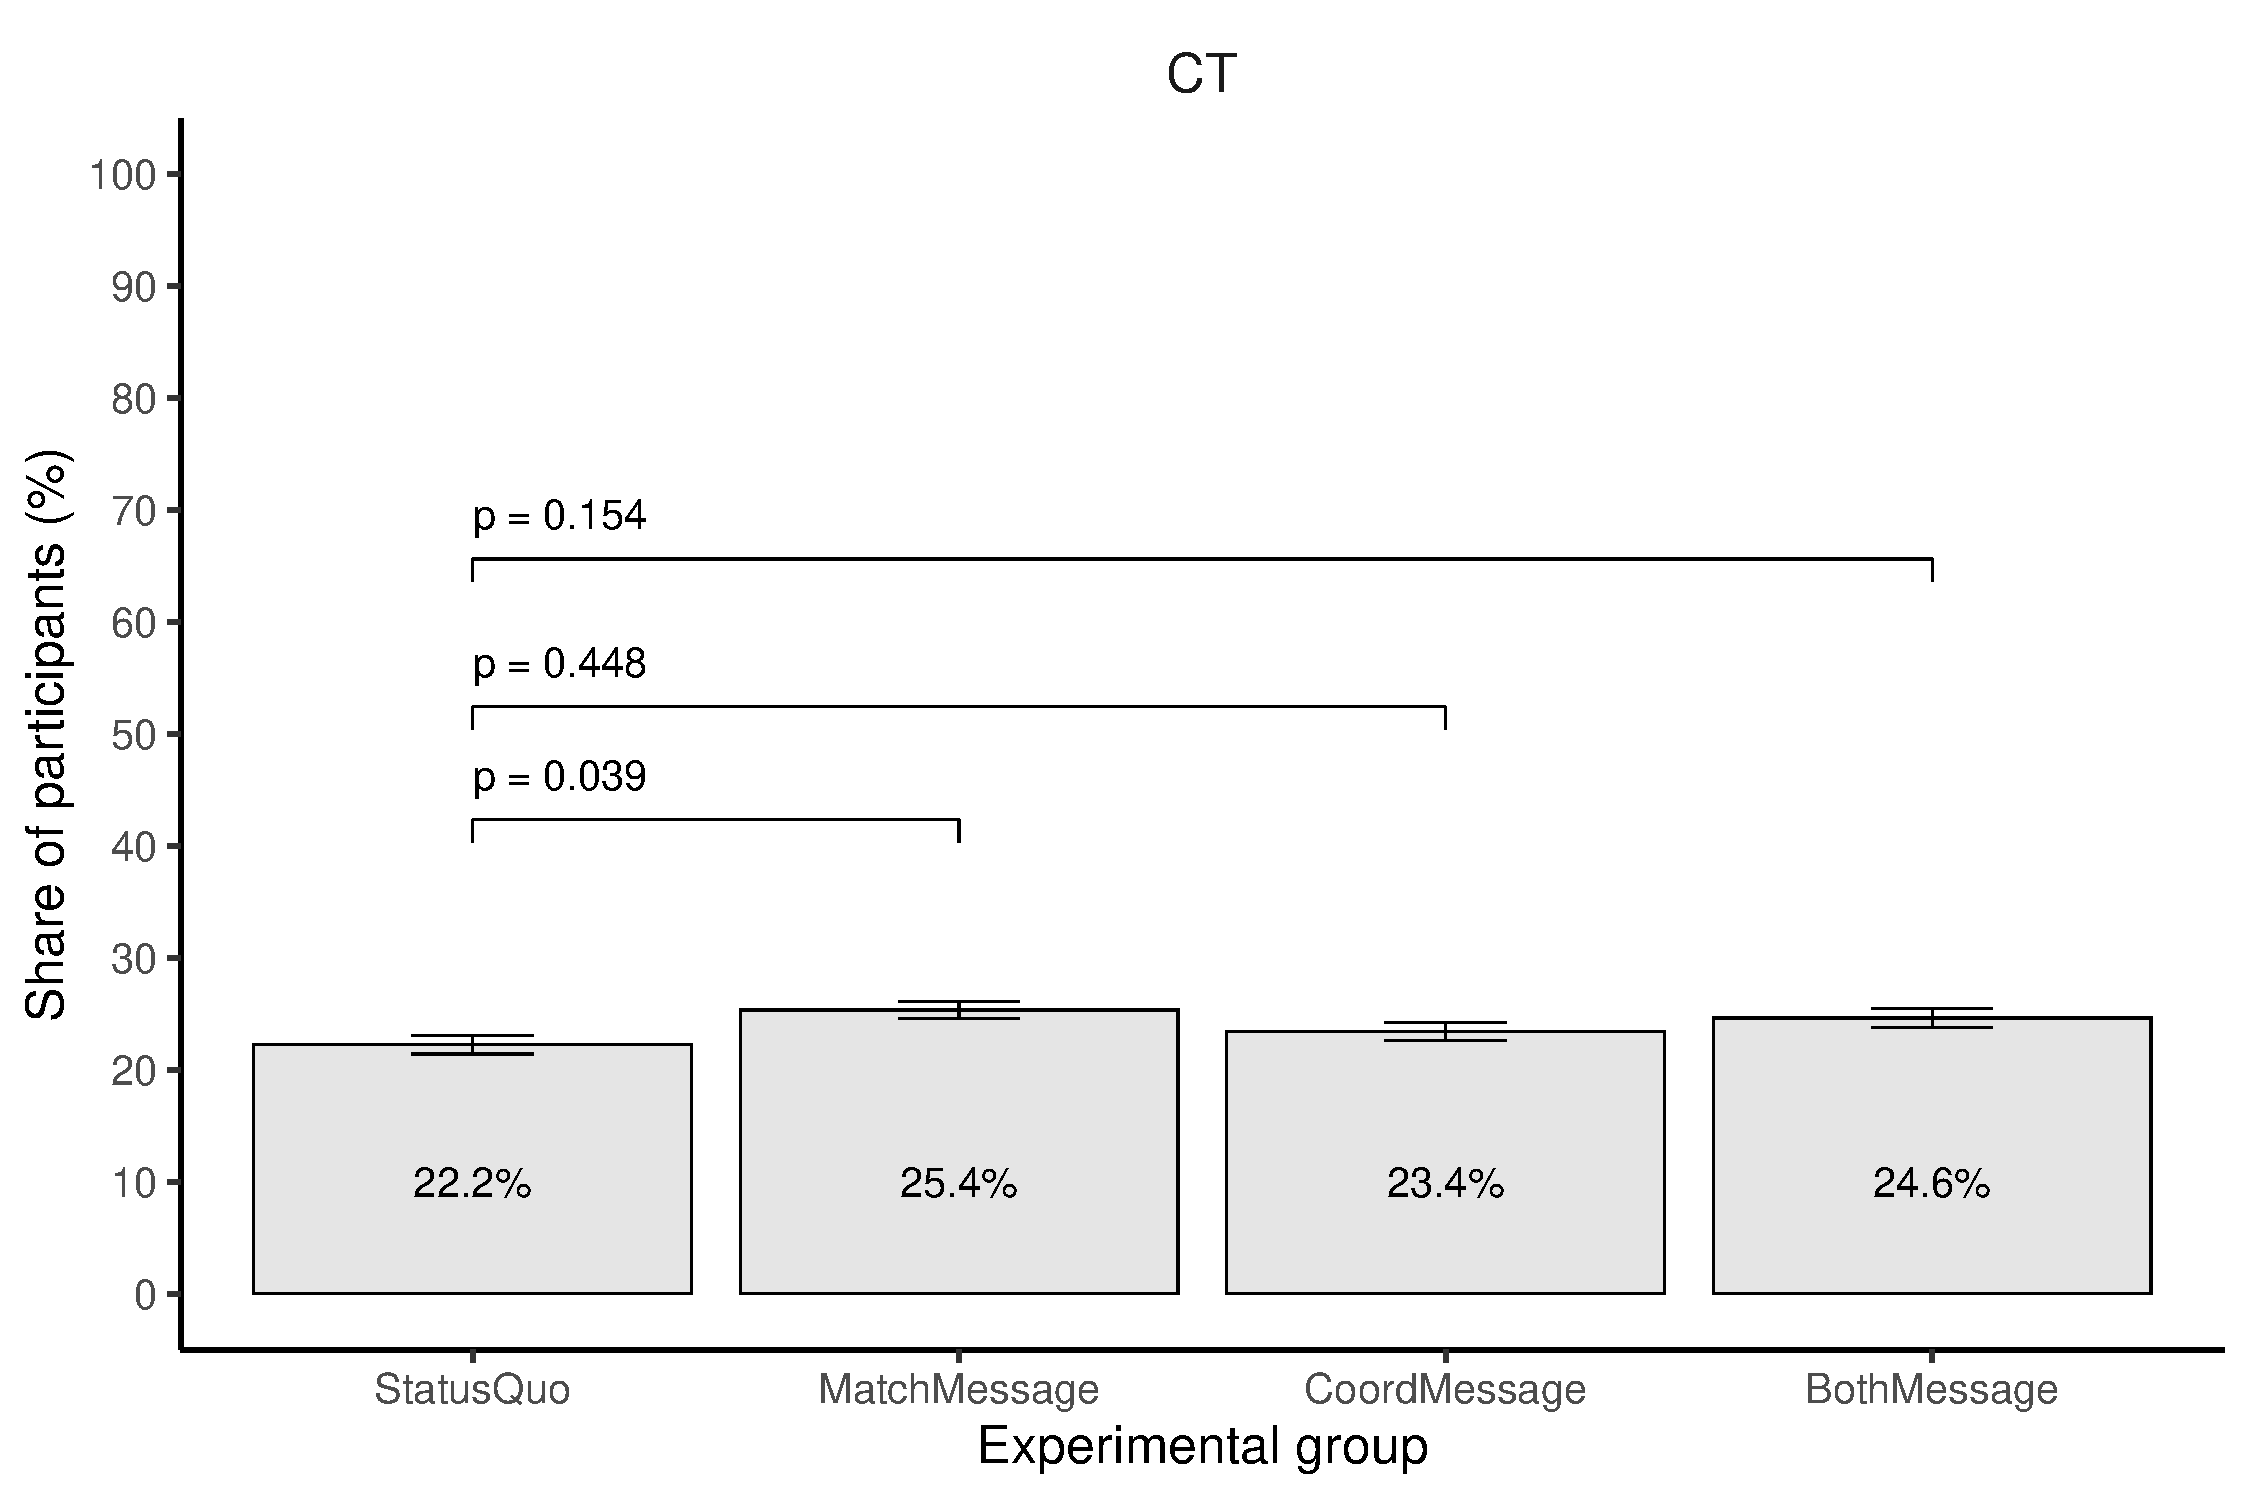
\includegraphics{JMDPRC~2/figure-latex/test-diff-mean-1} \caption{Sample Proportion of Reaching CT by Treatments.\newline \emph{Note}: Error bars show standard errors of the mean. For the statistical test, we used robust standard errors.}\label{fig:test-diff-mean}
\end{figure}

\begin{table}

\caption{\label{tab:lm-test}Linear Probability Model of the CT}
\centering
\fontsize{8}{10}\selectfont
\begin{threeparttable}
\begin{tabular}[t]{>{\raggedright\arraybackslash}p{20em}cc}
\toprule
\multicolumn{1}{c}{ } & \multicolumn{2}{c}{CT} \\
\cmidrule(l{3pt}r{3pt}){2-3}
  & (1) & (2)\\
\midrule
Treatment B & \num{3.10}*** & \num{2.56}**\\
 & (\num{1.14}) & (\num{1.16})\\
Treatment C & \num{1.19} & \num{0.50}\\
 & (\num{1.16}) & (\num{1.07})\\
Treatment D & \num{2.39}** & \num{1.64}\\
 & (\num{1.17}) & (\num{1.08})\\
\midrule
\addlinespace[0.3em]
\multicolumn{3}{l}{\textit{Adjustment of p-values for Multiple Testing}}\\
\hspace{1em}Treatment B & 0.021 & \\
\hspace{1em}Treatment C & 0.311 & \\
\hspace{1em}Treatment D & 0.073 & \\
Control average & 22.25 & 22.25\\
Covariates &  & X\\
Num.Obs. & \num{11049} & \num{11049}\\
RMSE & \num{23.79} & \num{29.00}\\
\bottomrule
\end{tabular}
\begin{tablenotes}
\item \emph{Note}: * $p < 0.1$, ** $p < 0.05$, *** $p < 0.01$. The robust standard errors are in parentheses. The unit of treatment effect is a percentage point. Covariates are gender, age, its squared term, the number of past coordinations, the number of public holidays in the assigned week and the following week, the number of hospitals per 10 square kilometers, the number of hospitals with PBSC collection per 10 square kilometers, the number of hospitals with BM collection per 10 square kilometers, and a dummy indictating that candidate can have skipped the CT. All covariates except gender dummy and dummy of skipped CT were demeaned. To adjust p-values for multiple testing, we employed the method proposed by \citet{List2019}. For calculation of p-values, we used the bootstrapping with 3,000 bootstrap samples.
\end{tablenotes}
\end{threeparttable}
\end{table}

We show the proportion of donors reaching CT by experimental arm in Figure \ref{fig:test-diff-mean}. This figure shows that experimental arms B and D, which include the probability message, increased the probability of reaching CT by 3.1 and 2.4 percentage points, respectively. These effects were statistically significant. We obtained the same results when we adjusted for multiple testing as proposed by \citet{List2019} (see column (1) of Table \ref{tab:lm-test}). When controlling for covariates in a linear probability model, the effect of experimental arm B remained statistically significant (see column (2) of Table \ref{tab:lm-test}). However, the effect of experimental arm D was statistically insignificant. This is due to a slight imbalance in cases eligible for skipping CT between experimental arm D and the control arm. In JMDP coordination, CT can be skipped when the previous CT remains valid.\footnote{Almost all candidates whose CT was skipped (except for one candidate) had prior coordination experience.} In fact, while the proportion of potential donors with prior coordination experiences in experimental arm D was not higher than in the control arm, it was statistically significant at the 10\% level in increasing the probability of CT being skipped (see Table A3 in Supplementary Material A). This difference likely influences the simple mean difference between experimental arm D and the control arm. These results are robust to using logistic regression models instead of linear probability models (see Table A4 in Online Supplementary Material A). In summary, the probability message included in experimental arm B increased the probability of reaching CT.

As mentioned earlier, our interventions were expected to increase the probability of reaching CT through improving willingness to donate and preventing dropouts between response and CT. Therefore, we decompose the message effects into three components: responses with willingness to donate, prevention of attrition due to patient-side reasons (exogenous attrition), and prevention of attrition due to donor-side reasons (endogenous attrition). We call attrition due to patient-side reasons ``exogenous attrition'' because it occurs due to factors outside donors' decision-making. We present these results in Table A5 in Supplementary Material A. The sum of the effects on these three factors is equal to the overall message effects on CT completion. While these effects were not statistically significant, after controlling for covariates, the probability message that increased the CT completion rate could have contributed to both improving and maintaining willingness to donate. In particular, the probability message relatively contributed more to improving willingness to donate, which accounts for half of the effect on reaching CT.\footnote{We divided the effect of experimental arm B on responses with willingness to donate by the sum of absolute values of the effects on three factors (\(3.44\) for experimental arm B).}

The early coordination message included in experimental arm C was expected to increase the CT completion rate through encouraging early responses. Indeed, among donors who indicated willingness to donate, those who responded earlier had a higher probability of reaching CT (see Figure A1 in Supplementary Material A). Therefore, we examine whether experimental arm C, while not increasing overall willingness to donate, increased early responses accompanied by willingness to donate. First, as visual evidence, we show the cumulative response rates with willingness to donate over time by experimental arm in Figure A2 in Supplementary Material A. Since JMDP requests responses within seven days, we define early responses as cumulative response rates with willingness to donate within seven days. However, experimental arm C did not have any effect on increasing the probability of responding with willingness to donate within seven days. This result was also confirmed by regression analysis (see Table A6 in Supplementary Material A). Therefore, the early coordination message did not have the effect we expected.

\hypertarget{heterogeneous-treatment-effects-on-ct}{%
\subsubsection{Heterogeneous Treatment Effects on CT}\label{heterogeneous-treatment-effects-on-ct}}

In this subsection, we explore the heterogeneity of message effects. First, we examine differences in effects by gender. Table A7 in Supplementary Material A presents estimation results from linear probability models that include cross terms between the male dummy and experimental arms.\footnote{In the cross-term models, we also controlled for cross terms between the male dummy and each covariate.} Without controlling for covariates, experimental arm D had a statistically significant positive effect on the probability of reaching CT for female potential donors. Furthermore, the cross term between this experimental arm and the male dummy was statistically significant at the 10\% level, suggesting that the effect of experimental arm D could be heterogeneous across gender. However, when controlling for covariates (including a dummy variable indicating whether CT was skipped), these results were not obtained. On the other hand, experimental arm B, which only included the probability message, did not have a statistically significant effect on the probability of reaching CT for female pontential donors but significantly increased the probability of reaching CT for mal potential donors. This result remained robust when controlling for covariates.

Next, we examine differences in effects between first-time matched donors and matched donors with prior coordination experience. Table A8 in Supplementary Material A presents estimation results from linear probability models that include cross terms between the first-time coordination dummy and experimental arms. The results show that experimental arm B had a statistically significant positive effect on the probability of reaching CT for potential donors with prior coordination experience. This result remained robust when controlling for covariates. However, none of the experimental arms had a statistically significant effect on the probability of reaching CT for first-time matched donors. To summarize these findings, the probability message included in experimental arm B primarily affects male potential donors who had prior coordination experience.

\hypertarget{process}{%
\subsection{Effects on the Coordination Process After CT}\label{process}}

Finally, we examined the effects of messages on subsequent stages of the coordination process after CT. As explained in Section \ref{background}, the coordination process comprises three stages: donor selection, final consent, and collection (donation). For these outcomes, we used dummy variables that take the value of 1 if a matched donor reached each stage. We analyzed the effects on post-selection stages, while acknowledging that these outcomes involve demand-side effects and thus require careful interpretation. In the control arm, \(6.2\)\% of potential donors were selected as the most appropriate donors, and \(4.5\)\% ultimately donated.

\begin{figure}[t]
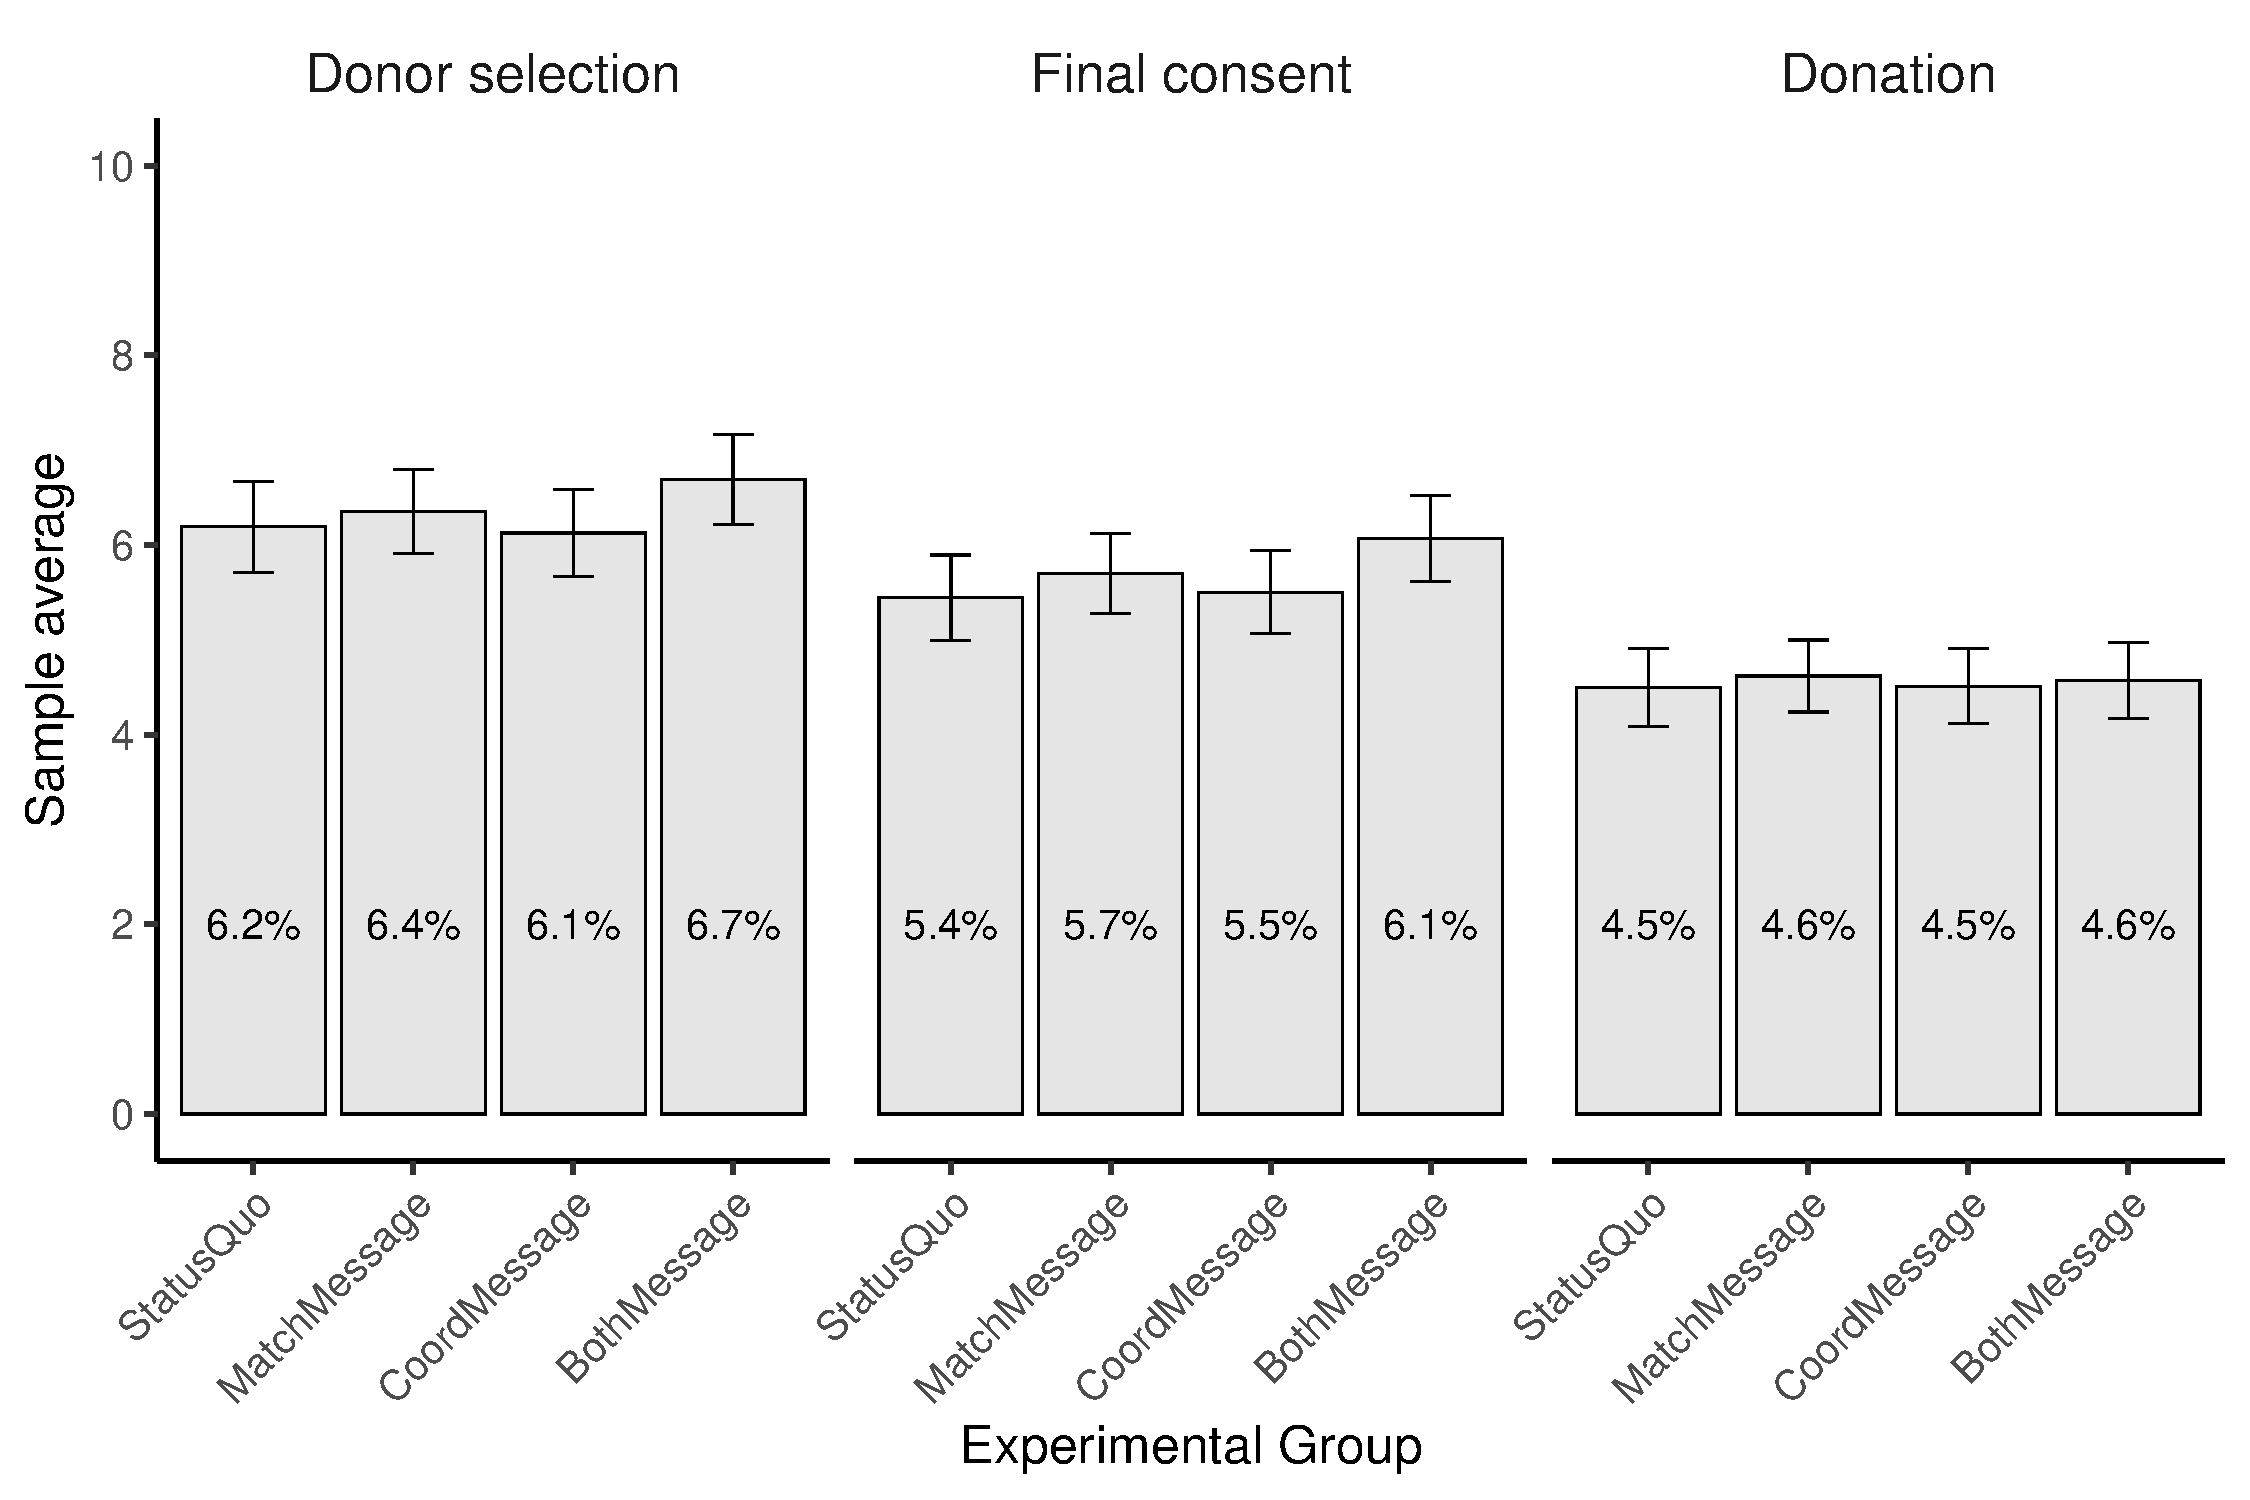
\includegraphics{JMDPRC~2/figure-latex/coordinate-diff-mean-1} \caption{Sample Averages of Donor Selection, Final Consent, and Donation by Treatments.\newline \emph{Note}: Error bars show standard errors of the mean. For the statistical test, we used robust standard errors.}\label{fig:coordinate-diff-mean}
\end{figure}

\begin{table}

\caption{\label{tab:lm-coordinate}Linear Probability Model of Coordination Process After CT}
\centering
\fontsize{8}{10}\selectfont
\begin{threeparttable}
\begin{tabular}[t]{lcccccc}
\toprule
\multicolumn{1}{c}{ } & \multicolumn{2}{c}{Donor selection} & \multicolumn{2}{c}{Final consent} & \multicolumn{2}{c}{Donation} \\
\cmidrule(l{3pt}r{3pt}){2-3} \cmidrule(l{3pt}r{3pt}){4-5} \cmidrule(l{3pt}r{3pt}){6-7}
  & (1) & (2) & (3) & (4) & (5) & (6)\\
\midrule
Treatment B & \num{0.16} & \num{-0.29} & \num{0.26} & \num{-0.14} & \num{0.12} & \num{-0.12}\\
 & (\num{0.65}) & (\num{0.69}) & (\num{0.62}) & (\num{0.66}) & (\num{0.56}) & (\num{0.61})\\
Treatment C & \num{-0.07} & \num{-0.32} & \num{0.06} & \num{-0.16} & \num{0.02} & \num{-0.15}\\
 & (\num{0.66}) & (\num{0.65}) & (\num{0.63}) & (\num{0.62}) & (\num{0.57}) & (\num{0.57})\\
Treatment D & \num{0.50} & \num{0.26} & \num{0.63} & \num{0.43} & \num{0.07} & \num{-0.08}\\
 & (\num{0.68}) & (\num{0.67}) & (\num{0.64}) & (\num{0.64}) & (\num{0.57}) & (\num{0.57})\\
\midrule
Control average & 6.19 & 6.19 & 5.44 & 5.44 & 4.50 & 4.50\\
Covariates &  & X &  & X &  & X\\
Num.Obs. & \num{11049} & \num{11049} & \num{11049} & \num{11049} & \num{11049} & \num{11049}\\
RMSE & \num{6.30} & \num{7.97} & \num{5.64} & \num{7.07} & \num{4.50} & \num{5.55}\\
\bottomrule
\end{tabular}
\begin{tablenotes}
\item \emph{Note}: * $p < 0.1$, ** $p < 0.05$, *** $p < 0.01$. The robust standard errors are in parentheses. The unit of treatment effect is a percentage point. Covariates are gender, (demeaned) age, its squared term, the number of past coordinations, the number of public holidays in the assigned week and the following week, the number of hospitals per 10 square kilometers, the number of hospitals with PBSC collection per 10 square kilometers and the number of hospitals with BM collection per 10 square kilometers. All covariates except gender were demeaned.
\end{tablenotes}
\end{threeparttable}
\end{table}

We show sample averages of each outcome by experimental arm in Figure \ref{fig:coordinate-diff-mean}. No experimental arm affected the post-donor selection process. Similar results were obtained from linear probability models (see Table \ref{tab:lm-coordinate}) and logistic regressions controlling for covariates (see Table A9 in Online Supplementary Material A). These results should be interpreted with caution. Given that our intervention does not affect demand (number of patients), if our intervention increases the number of donors who reach CT, it should increase the number of donors who are not selected as candidates for exogenous reasons. In particular, compared to the control arm, experimental arm B increased by \(4.3\) percentage points the probability that potential donors who reached CT were not selected due to patient-related reasons or donor health conditions. This difference is statistically significant at the 10\% level (\(p = 0.095\)). Thus, the intervention effects are weakened by demand-side factors.

\hypertarget{conclusion}{%
\section{Discussion and Conclusions}\label{conclusion}}

This study examines how information provision affects the number of donors from whom physicians can select the optimal donor for transplantation. The results of field experiment show that information about the low number of HLA-matched donors per patient (probability message) increased the probability of reaching CT by improving and maintaining willingness to donate.

How many additional registrants does the increase in the probability of reaching CT due to the probability message correspond to? The probability message increased the probability of reaching CT by \(12\% (= 2.56/22.25)\). This is equivalent to increasing the number of registrants who match with patients and start coordination by 12\%.\footnote{Let \(N_m\) be the number of registrants who start coordination. Let \(N_1(d)\) be the number of potential donors who reach CT under treatment \(d\). Then, \(N_1(d) = p(d)N_m\) holds, where \(p(d)\) is the probability of reaching CT under treatment \(d\). Note that \(d = 1\) and \(d = 0\) represents a treatment arm and a control arm, respectively. We solve \(N_1(1) = p(0)[N_m + \Delta N_m]\) for \(\Delta N_m\), where \(\Delta N_m\) represents the increase in registrants who start coordination. As a result, we obtain \([p(1) - p(0)]/p(0) = \Delta N_m/N_m\).} In JMDP, 40\% of registrants become matched donors who start coordination\footnote{The cumulative number of registrants since JMDP's establishment is \(980,000\). Among them, \(390,000\) have become potential donors who started coordination. Thus, 40\% of registrants become potential donors who start coordination. Data source: \url{https://www.bs.jrc.or.jp/bmdc/donorregistrant/m2_03_00_statistics.html} (Japanese. Accessed December 8, 2024).}. With JMDP's current registrant pool of \(560,000\), the estimated number of potential donors is \(224,000\).\footnote{\url{https://www.bs.jrc.or.jp/bmdc/donorregistrant/m2_03_00_statistics.html} (Japanese. Accessed December 8, 2024).} Therefore, the effect of the probability message is equivalent to increasing the number of matched donors who start coordination from \(224,000\) to \(250,000 (= 224,000 \times 1.12)\), an increase of \(26,000\). In terms of registrants, the effect of the probability message is equivalent to increasing registrants from 560,000 to \(630,000 (= 560,000 \times 1.12)\), an increase of \(70,000\). In JMDP, the age limit for registration is 54 years old. Currently, there are approximately \(100,000\) registrants in their 50s, so JMDP's registrant pool will decrease by \(100,000\) over the next five years.\footnote{\url{https://www.jmdp.or.jp/about/read/number/} (Japanese. Accessed December 8, 2024).} Therefore, introducing the probability message could help mitigate the negative impact of registrant pool shrinkage due to aging.

The effects of the probability message were primarily observed among male potential donors with prior coordination experience. Recent review paper have discussed that when multiple potential donor options are available, physicians prefer male potential donors because patients with male donors are less likely to develop GVHD, a major complication of HSCT, and PBSC collection from male donors yields a higher cell count than from female donors \citep{Fingrut2018}.\footnote{GVHD is a phenomenon in which donor-derived lymphocytes mistakenly identify the patient's normal cells as foreign and attack them. This can lead to fever, skin symptoms, gastrointestinal symptoms such as diarrhea, and liver damage that may cause impaired consciousness.} In Japan, there is evidence that female donors with childbirth experience increase the risk of non-relapse mortality compared to male donors \citep{Shinohara2017}. In our data, among those who completed CT, male donors were more likely to be selected than female donors (see Table A10 in Supplementary Material A). Given these findings, the probability message likely improves coordination efficiency by promoting CT completion among male potential donors.

Why was treatment arm D, which included the probability message, not effective? The difference between treatment arms B and D is whether they presented the early coordination message, which did not significantly increase the probability of reaching CT. Therefore, treatment arm D includes not only the positive effect of the probability message but also the negative effect of information overload from simultaneously presenting the ineffective early coordination message, resulting in no statistically significant increase in the probability of reaching CT. There are two potential mechanisms for the positive effect of the probability message. First, it corrects optimistic beliefs about the number of alternative donors, thereby reducing free-riding incentives. Second, it makes the rarity of donation opportunities more salient. Unfortunately, we cannot characterize which mechanism caused the probability message to influence behavior.

This study has a practical implication. The findings suggest that information provided by the program office to registrants at the time of matching with patients can promote behavioral changes in a desirable direction. However, given that some studies have shown that information provision is ineffective \citep[e.g.,][]{Switzer2018}, the effectiveness of our information provision protocol should be tested in bone marrow donor programs in other countries.

\clearpage

\bibliography{biblio.bib}



\end{document}
